\chapter{Introduction and problem statement}
\label{cha:intro}
With the enormous amount of data we produce nowadays, data mining is becoming more and more prevalent.
Consequently, the goal with modern data mining methods is not only to discover information from crude data, but also to condense that information down to concise descriptions and insights.
One such method is redescription mining~\citep{ramakrishnan_turning_2004}.
In a nutshell, it aims to find different ways to describe the same things.

\chapter{Background Knowledge}
\label{cha:background}
In this chapter we are going to explore the underlying theory of the thesis.
We will go from more general knowledge to more specific concepts.
Firstly, the data mining concepts and framework are introduced.
Data mining is the process of extracting information from raw data.
Then we will dig deeper into frequent itemset mining and redescription mining, which are the two main tasks that the thesis is built upon.

\section{Data mining}
\label{sec:datamining}
Why did data mining was developed?
This chapter can give some context about that and then introduces some building blocks of the data mining framework.
\subsection{The problems}
\label{sub:the_problems}
The invention of the computer changed the way we think about storing and managing data.
Unlike books in the library or merchants in the store, data in computers can grow exponentially and instantaneously at a rate like never before.
The need for a systematic way to collect and extract useful information from a big data set started to coin in the late 1980s within companies' research departments \citep{coenen_datamining_2011}.

One of the first problems that data mining tried to solve is to create decision supports from retail clients' transactions and the sales information \citep{coenen_datamining_2011}.
The aim is to drive the sales up, by giving out suggestions, promotions, and special pricing to the targeted customer based on their behaviors.
For example, retailers can use the system to find out which items are frequently bought together, then arrange them close to each other to create a reminding effect, which can increase the sale.
Advance a few decades later, Netflix - a streaming service company - created a system to recommend movies to users based on their favorites and activities \citep{netflix_rs_2016}.
The most difficult part of such a system is that the data is often significantly smaller than the search space.
An average person can only watch a limited number of movies, while the total number of movies is vastly bigger.
Along with that, nowadays, with the raising of low-cost communicable devices and sensors, we need to find efficient ways to deal with the data produced by them \citep{data_mining_iot_2014}.
Hence, more sophisticated and clever methods are needed; and many have been invented to deal with the growing of the complexities of the problems.

These are just a few examples of some problems that emerged in the modern time of computing and data mining.
As we can imagine, the potential of data mining is unbounded.

\subsection{The main building blocks}
\label{sub:building_blocks}

There are three main phases of data mining: \textit{data collection}, \textit{data wrangling}, and \textit{analytical processing}.

Data collection usually involves the use of hardware or software to acquire raw data.
This could be sensors' data of the environment, or user activities data from computer applications.
The choice of which data to collect is crucial and can affect greatly the quality of the result in the later phases.

After the data is collected, it is usually in a form that is difficult to be processed directly by the algorithms.
That's why we need the data preprocessing phase to make the data easier to be consumed.
This could be structuring the data into known format, e.g. multidimensional formats, time series, etc.; or removing corrupted data.

Analytical processing is the most interesting phase where useful information or insights start to emerge.
From the analytical perspective, we can categorize data mining into four "super problems": clustering, classification, \ac{apm} and outlier analysis \citep{Aggarwal15}.
Even though mining processes are different from each other, they often share some similarities and common patterns that we can generalize and apply similar techniques to them.
For example, association patterns are somewhat similar to overlapping clusters, where each pattern is corresponding to a cluster.

In the scope of this thesis, we will be more interested on the \acl{apm} problem.
\Acl{fim} \citep{borgelt_fim_2012} is the most popular model of \acl{apm}.

% Maybe introduce more type of problems here (Aggarwal15 4.1)

\section{\Acl{fim}}
\label{sec:fim}
\Acl{fim} was originally developed for marketing purposes introduced in \autoref{sub:the_problems}.
The initial goal was to analyze the market basket data to extract information about which items are frequently bought together.
Nowadays, the applications of \acl{fim} expanded to many more domains, with different kind of tasks.

\subsection{Definitions}
\label{sub:association_rule_mining}
\begin{table}[tb]
    \centering
    \begin{tabular}{|l|c|c|}
        \hline
        \textbf{tid} & \textbf{Transaction}                           & \textbf{Binary representation} \\ \hline
        T101         & \{I1: Bread\}                                  & \texttt{1000}                  \\ \hline
        T102         & \{I2: Butter\}                                 & \texttt{0100}                  \\ \hline
        T103         & \{I3: Jam\}                                    & \texttt{0010}                  \\ \hline
        T104         & \{I4: Milk\}                                   & \texttt{0001}                  \\ \hline
        T105         & \{I1: Bread, I3: Jam\}                         & \texttt{1010}                  \\ \hline
        T106         & \{I1: Bread, I2: Butter, I3: Milk, I4: Jam\}   & \texttt{1111}                  \\ \hline
    \end{tabular}%
    \caption{An example of market basket dataset in binary representation}
    \label{tab:binary-prepresentation}
\end{table}
Formally, assume that we have a universe of all possible items $\universeOfItemset$.
For example, this can be all the possible products in a groceries store.
Suppose we have a set of $\mathit{n}$ transactions $\transaction{} = \transactionDef{}$, where $\transaction{i}$ is a composition of items from $\universeOfItemset$, with $i$ is the \ac{tid}.
This in turn, could be possible transactions at a groceries store.
Intuitively, the size of $\universeOfItemset$ is usually much larger than the size of $\transaction{}$.

Such a collection of transactions can be represented in binary representation, where all records have the same length, and each record represents a transaction.
One item in $\universeOfItemset$ will have it own same position in all records.
We can see that the length of each record is basically $|\universeOfItemset|$.
If an item appears in a transaction, it will have value $1$ in the corresponding record, otherwise $0$.
We can see this in the example \autoref{tab:binary-prepresentation}, for the first row, only I1 was present in the transaction, hence in the binary representation of the transaction, the first position, which corresponding to I1, is set to $1$.
This representation is analogous to a matrix where the rows are the records and represents the transactions, and the columns correspond to the items.
The presence of the $\mathit{j}$th item in the $\mathit{i}$th transaction is recorded as the value in cell $\mathit{(i, j)}^{th}$.

A set of items in $\universeOfItemset$ is an \textit{itemset}.
We refer to a set of $k$ items as \kItemset.
The \textit{support} of an itemset is the set of transactions which contains the itemset.
We might also encounter an alternative way of defining \textit{support} in other literatures where it is defined as the frequency which an itemset appears in as a subset of a transaction in the dataset.
Let us agree that the notation \textit{support} in the scope of this thesis is referring to the first definition above, where the support is a set.
We will call the number of transactions in the that set \textit{support count}, and the fraction of the support count vs the number of all transactions frequency ($\mathit{freq}$): 
\begin{equation}
    \frequency{I} = \frac{\lvert\support{I}\rvert}{\lvert\transaction{}\rvert}
\end{equation}

\begin{definition}[Support]
    The support of an itemset $\itemset$ is defined as the set of transactions in the database $\transaction{} = \transactionDef{}$ that contains $\itemset$ as a subset.
    The support of itemset $\itemset$ is denoted by $\support{I}$.
\end{definition}
For example in \autoref{tab:binary-prepresentation}, $\support{\{I1, I3\}} = \{T105, T106\}$.
The frequency is calculated by $\frequency{\{I1, I3\}}=2/6=0.(3)$.
The aim of \acl{fim} is to find the itemsets with support count above a predefined \ac{minsup}.

\begin{definition}[\Acl{fim} \citep{Aggarwal15}]
    Given a set of transactions $\transaction{} = \transactionDef{}$, where each transaction $\transaction{i}$ is a subset of items from $\universeOfItemset$, determine all itemsets $\itemset$ that occur as a subset of at least a predefined $\minsup$ of the transactions in $\transaction{}$.
\end{definition}

In addition to normal frequent itemset, there are two useful extended concepts of frequent itemset: closed frequent itemset and maximal frequent itemset.
An itemset $X$ is closed, if none of its supersets have exactly the same support count as $X$~\cite{Aggarwal15}.
A closed frequent itemset is an itemset that is both closed and frequent.
\begin{definition}[Closed frequent itemset ]
    With $Y$ is an itemset and $X$ is a frequent itemsets, $X$ is a closed frequent itemset if:
    \begin{equation}
        \forall Y \supset X, \supportcount{Y} < \supportcount{X}
    \end{equation}
\end{definition}

A frequent itemset is maximal if none of it superset is frequent~\cite{Aggarwal15}.

\begin{definition}[Maximal frequent itemset]
    Let $F$ is the set of all frequent itemsets in a dataset. $X$ is a frequent itemset in $F$. $X$ is maximal frequent itemset if:
    \begin{equation}
        \nexists Y \in F \mid X \in F \wedge X \subset Y
    \end{equation}
\end{definition}

There are several observations we can make here:
\begin{itemize}
    \item Let $F$ is the set of all frequent itemsets, $C$ is the set of all closed frequent itemsets, and $M$ is the set of all maximal frequent itemsets. $M \subseteq C \subseteq F$.
    \item Closed frequent itemsets keep all the information, such as supports of the subsets. In other words, we can restore the supports of any frequent itemset from the closed frequent itemsets.
    \item Maximal frequent itemsets do not keep all information about all the frequent itemsets. We only know that all of their subsets are frequent, but we cannot determine their supports.
\end{itemize}

\Ac{fim} is the first phase of \ac{arm}.
In the following phase, the output of \ac{fim} can be further processed to find the association rules with \acl{arm}.
The result of this step is a set of rules that can be used to predict the behavior of the users.
For example, we can come to a finding that people who buy beer might also buy diapers.
Such strange finding is not quite trivial to thought of, but with the help of \acl{arm}, we can obtain it.

In order to determine whether a rule is trustworthy or not, we need to introduce a new measure: confidence.
The confidence of a rule $X \Rightarrow Y$ is the fraction of transactions containing $X$, which also contain $Y$.
\begin{definition}[Confidence \citep{Aggarwal15}]
    Let $X$ and $Y$ be two set of items.
    The confidence $\confident{X}{Y}$ of the rule $X \Rightarrow Y$ is the conditional probability of $X \cup Y$ occurring in a transaction, given that the transaction contains $X$.
    Therefore, the confidence $\mathit{conf}(X \cup Y)$ is defined as follows:
    \begin{equation}
        \confident{X}{Y} = \frac{\supportcount{X \cup Y}}{\supportcount{X}}
    \end{equation}
\end{definition}
In other words, the confidence of a rule $X \Rightarrow Y$ is the conditional probability that a transaction contains the itemset $Y$, given that it contains the itemset $X$.

For example in \autoref{tab:binary-prepresentation}, the support of \{I1, I3\} is $\support{\{I1, I3\}} = \{T105, T106\}$.
And the support of \{I1, I2, I3, I4\} is $\support{\{I1, I2, I3, I4\}} = \{T106\}$.
Hence, the confidence of the rule $\text{\{I1, I3\}} \Rightarrow \text{\{I2, I4\}}$ is $1 / 2 = 0.5$.

Now since we have the confidence, the definition of an association rule can be presented as follows:
\begin{definition}[Association rules \citep{Aggarwal15}]
    Let $X$ and $Y$ be two sets of items.
    The rule $X \Rightarrow Y$ is said to be valid at support level $s$ and confidence level $c$, if the following conditions are satisfied:
    \begin{enumerate}
        \item The support of the item set $X$ is at least $s$;
        \item The confidence of $X \Rightarrow Y$ is at least $c$;
    \end{enumerate}
    The first criterion ensures that a sufficient number of transactions are relevant to the rule; therefore, it has the required critical mass for it to be considered relevant to the application at hand.
    The second criterion ensures that the rule has sufficient strength in terms of conditional probabilities.
    Thus, the two measures quantify different aspects of the association rule.
\end{definition}
As we can see the confidence together with the minimum support are the core parameters of \acl{arm}.
The minimum support is used in the first phase of \acl{arm} to determine the frequent itemsets.
And the minimum confidence is used in the second phase to determine the association rules.

The frequent itemset mining phase usually takes up most of the computation time of the whole process.
Therefore, most of the research work is focused on it.
\subsection{The search space}
\label{sub:search_space}
% Let us use the \acl{ne} to go through it and see what will happen.
% Even though the \acl{ne} does not have any practical application, using it helps us to understand the computational complexity of \ac{fim} problem and appreciate the benefit of some optimization techniques. %, e.g. pruning or efficient support counting.

% The \acl{ne} is, unsurprisingly, very simple. It tries to check all the possible combinations to see if one is a frequent itemset or not.
% For example, with the universe of 4 items, all the possible combinations of items are represented in \autoref{fig:item-lattice}.
% In order to check the frequency of an itemset, we need to count the number of transactions that contain the itemset, this step is called \textit{support counting}.
The search space of \acl{fim} problem is enormous.
Considering a universe of items $\universeOfItemset$, there will be a total of $2^{\left\lvert \universeOfItemset \right\rvert} - 1$ possible combinations, or itemsets, excluding the empty set.
In other words, the size of the possible itemsets grows exponentially with the size of the universe.
To put this into perspective, a universe of 100 items will have a total of $2^{100} - 1$ possible itemsets, which is bigger than $10^{30}$.
At the time of writing this, the most powerful supercomputer is the Fugaku with the speed of approximately 0.4 exaflop/s \citep{monroe_fugaku_2020}.
Suppose we use this supercomputer to enumerate through the search space of all $10^{30}$ possible itemsets, and each iteration will cost us 1 flop, even though most likely it will cost more than that; this whole process will then take at least $2.5^{12}$ seconds, or at least 79 thousands years.
And all that was just for enumerating the search space, we are supposed to do the support counting at each stop and that will take much more time than the enumeration.
Realistically, the size of $\universeOfItemset$ is often much bigger than 100.
To say the least, this \acl{ne} is not practical, even for datasets over small collections of items.
There are several optimization techniques that we will discover in the following subsection.

% We will discuss some properties that can be used to optimize the frequent itemset mining phase in \autoref{sub:apriori }.
\subsection{The \acl{apriori}}
\label{sub:apriori}
\begin{figure}
    \centering
    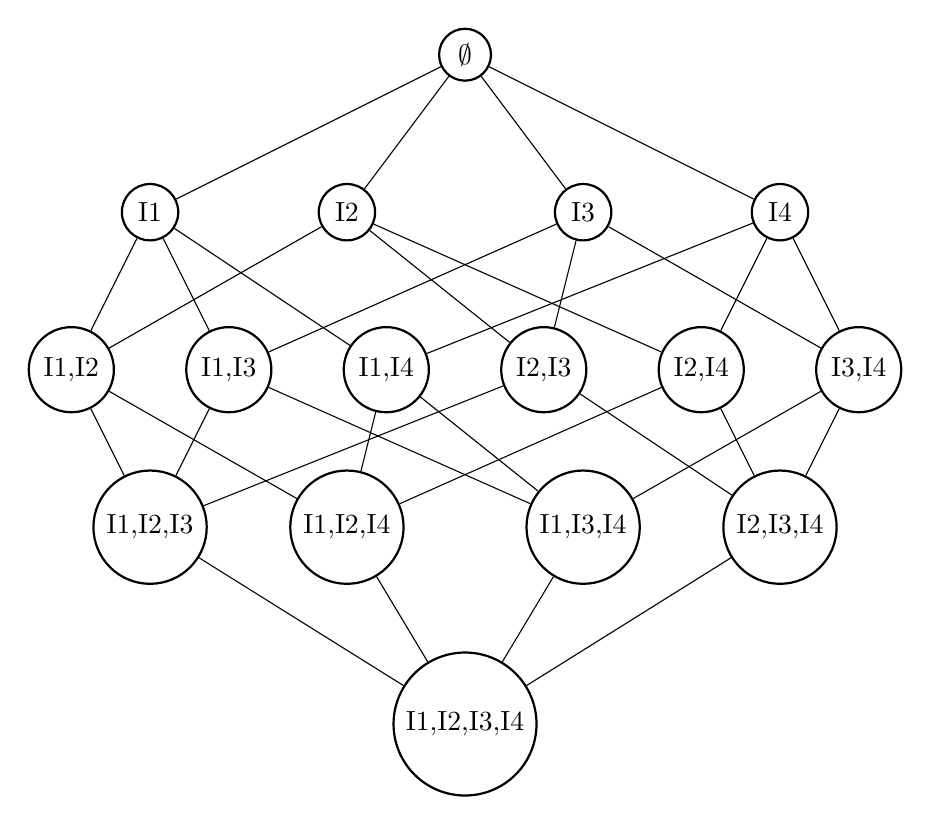
\begin{tikzpicture}[y=-1cm]
        \begin{scope}[every node/.style={circle,thick,draw}]
            \node (E) at (5,0) {$\emptyset$};
            \node (A) at (1,2) {I1};
            \node (B) at (3.5,2) {I2};
            \node (C) at (6.5,2) {I3};
            \node (D) at (9,2) {I4};
            \node (AB) at (0,4) {I1,I2};
            \node (AC) at (2,4) {I1,I3};
            \node (AD) at (4,4) {I1,I4};
            \node (BC) at (6,4) {I2,I3};
            \node (BD) at (8,4) {I2,I4};
            \node (CD) at (10,4) {I3,I4};
            \node (ABC) at (1,6) {I1,I2,I3};
            \node (ABD) at (3.5,6) {I1,I2,I4};
            \node (ACD) at (6.5,6) {I1,I3,I4};
            \node (BCD) at (9,6) {I2,I3,I4};
            \node (ABCD) at (5,8.5) {I1,I2,I3,I4};
        \end{scope}
        \draw (E) -- (A);
        \draw (E) -- (B);
        \draw (E) -- (C);
        \draw (E) -- (D);
        \draw (A) -- (AB);
        \draw (A) -- (AC);
        \draw (A) -- (AD);
        \draw (B) -- (AB);
        \draw (B) -- (BC);
        \draw (B) -- (BD);
        \draw (C) -- (AC);
        \draw (C) -- (BC);
        \draw (C) -- (CD);
        \draw (D) -- (AD);
        \draw (D) -- (BD);
        \draw (D) -- (CD);
        \draw (AB) -- (ABC);
        \draw (AB) -- (ABD);
        \draw (AC) -- (ABC);
        \draw (AC) -- (ACD);
        \draw (AD) -- (ABD);
        \draw (AD) -- (ACD);
        \draw (BC) -- (BCD);
        \draw (BC) -- (ABC);
        \draw (BD) -- (ABD);
        \draw (BD) -- (BCD);
        \draw (CD) -- (ACD);
        \draw (CD) -- (BCD);
        \draw (ABC) -- (ABCD);
        \draw (ABD) -- (ABCD);
        \draw (ACD) -- (ABCD);
        \draw (BCD) -- (ABCD);
    \end{tikzpicture}
    \caption{The item lattice for a universe of 4 items.}
    \label{fig:item-lattice}
\end{figure}

As we just saw, the search space of itemsets is huge.
Hence, it is not reasonable to enumerate all possible itemsets, since a lot of candidates are inefficiently generated by the algorithm for each iteration.
Instead, we need some better strategy for traversing it.

A sensible approach to improve this is to reduce the search space by pruning some candidates, or better not generating those that we know they will not be frequent.
We know that if an itemset $I$ exists in a transaction, then all of its subsets $X_1, X_2, \dots, X_k$ must also exist in the transaction.
Hence, the number of transactions that one subset $X_i$ can be found in is always larger or equal to the corresponding value of the itemset $I$.
This is called the \acl{smp}:
\begin{definition}[\Acl{smp} \citep{Aggarwal15}]
    The support count of every subset $X$ of $Y$ is at least equal to that of the support count of itemset $Y$.
    \begin{equation}
        \supportcount{X} \geq \supportcount{Y} \quad \forall X \subseteq Y
    \end{equation}
\end{definition}

The direct implication from the \acl{smp} is that every subset $X_i$ of a frequent itemset $Y$ is also frequent.
This is also called the \acl{dcp} \citep{Aggarwal15}.
We can apply this property in the opposite direction, that is, if a itemset $X$ is not frequent, then none of its supersets $Y_1, Y_2, \dots, Y_k$ can be frequent.
For example in the \autoref{fig:item-lattice}, if during the searching, we found out that $X = \{I1, I2\}$ is not frequent, then all the supersets of $X$, e.g. $\{I1, I2, I3\}, \{I1, I2 , I4\}, \{I1, I2 , I3, I4\}$, cannot be frequent.
We can then drop all supersets of ${Y = \{I1, I2\}}$ from the search space.
This is a huge advantage since it allows us to stop searching early for all the supersets if we know that one of the subsets is not frequent.
What we have here is essentially the core of the \acl{apriori}, where the \acl{dcp} is applied to a \ac{ne}.
By utilizing the simple \acl{dcp} property above, the amount of candidates we have to process is drastically reduced.

% TODO add pseudo code here

The family of algorithms that enumerate the search space horizontally (breadth-first search), in turn considering candidates of size $k$, iteratively increasing the value of $k$, i.e. proceed in a level-size manner, are called the \acl{lwa}.
The \acl{apriori} is one of the earliest and most popular \acl{lwa}.
There are also approaches those traverse the search space vertically, or in other words, in a depth-first search manner.
We will later study one of such algorithm: the \acl{fpg} in \autoref{sub:fp-growth}.
% Support counting is usually a very expensive task if done naively.
% Trying to count the support more efficiently is also a good way to improve the performance.
% In \citep{brin_et_al_1997}, the \ac{dic} algorithm was presented, where itemsets are dynamically added and deleted as transactions are read instead of waiting for the scanning of the whole dataset to be completed.
% This technique proposes a concept called count-so-far which is a lower bound of the actual count of the itemset.
% If the itemset's count-so-far value is bigger than the minimum support then it will be added to the frequent itemset collection.

% One approach to prune the search space is the hash-based technique \citep{Vanitha2011USINGHB}.
% In the hash-based technique, we first scan all the transactions, we will generate all the 2-itemsets candidates for each one.
% For each 2-itemsets, we hash it into a bucket in a hash table and increase the count of the bucket by 1 if it already exists.
% The result is a table indexed by the hash value of the 2-itemsets, and the value of each bucket is the number of transactions that contain the 2-itemsets.
% We then go through the table and prune the candidates that are not frequent, i.e. the count of the bucket is less than the minimum threshold.
% This approach can reduce the number of \kItemset s substantially, especially with 2-itemsets.

% We can also use some data structure to store the candidates and/or transactions in a way that can be used to count the support efficiently.
% For instance, in \citep{bodon2003fast}, a Trie data structure was used store the candidates so that we can quickly retrieve the supports of an itemset and generate the candidates.

% There are many more other approaches to further optimize the algorithm, such as Transaction reduction \citep{zhuang_2011_transaction_reduction}, Sampling (mining on a subset of the data) \citep{zaki_1991_sampling}, etc.


\subsection{Eclat}
\label{sub:eclat}
\begin{table}[]
    \centering
    \begin{tabular}{|l|l|c|}
        \hline
        \textbf{tid} & \textbf{Transaction}   & \textbf{Binary presentation} \\ \hline
        T001         & \{ I1, I2, I5 \}       & \texttt{11001}               \\ \hline
        T002         & \{ I2, I4 \}           & \texttt{01010}               \\ \hline
        T003         & \{ I2, I3 \}           & \texttt{01100}               \\ \hline
        T004         & \{ I1, I2, I4 \}       & \texttt{11010}               \\ \hline
        T005         & \{ I1, I3 \}           & \texttt{10100}               \\ \hline
        T006         & \{ I2, I3 \}           & \texttt{01100}               \\ \hline
        T007         & \{ I1, I3 \}           & \texttt{10100}               \\ \hline
        T008         & \{ I1, I2, I3, I5 \}   & \texttt{11101}               \\ \hline
        T009         & \{ I1, I2, I3 \}       & \texttt{11100}               \\ \hline
    \end{tabular}
    \caption{The transactional database in horizontal format \citep{han2012mining}}
    \label{tab:horizontal-transactional-database}
\end{table}

\begin{table}[]
    \centering
    \begin{tabular}{|l|l|c|}
        \hline
        \textbf{Items}   & \textbf{TID lists}                             & \textbf{Binary presentation} \\ \hline
        I1               & \{ T100, T400, T500, T700, T800, T900 \}       & \texttt{100110111}           \\ \hline
        I2               & \{ T100, T200, T300, T400, T600, T800, T900 \} & \texttt{111101011}           \\ \hline
        I3               & \{ T300, T500, T600, T700, T800, T900 \}       & \texttt{001011111}           \\ \hline
        I4               & \{ T200, T400 \}                               & \texttt{010100000}           \\ \hline
        I5               & \{ T100, T800 \}                               & \texttt{100000010}           \\ \hline
        \end{tabular}
    \caption{The transactional database in vertical format \citep{han2012mining}}
    \label{tab:vertical-transactional-database}
\end{table}

One big limitation of \acl*{apriori} is that it has to constantly scan the database to be able to count the supports.
The \ac{eclat} algorithm is an algorithm that does not require re-scanning the data repeatedly \citep{zaki1997}.

In \acl{apriori}, the data is in the horizontal format like in \autoref{tab:horizontal-transactional-database}, while \ac{eclat} works on vertical data format.
In the vertical transactional database, each itemset is now a key to a set of the transactions where it appears, like in \autoref{tab:vertical-transactional-database}.
In binary presentation, by transposing the horizontal data format,we will get the vertical data format.
The set of transactions is often called \ac{TID} set.
The importance of utilizing vertical data format is that we can find the support of an itemset by intersecting the \ac{TID} set of the children itemsets.

The next important concept of the \ac{eclat} algorithm is the \ac{ec}. The definition of \acl{ec} is defined as follow:

\begin{definition}[\Acl{ec} \citep{zaki2000}]
    Let $P$ be a set. An \textbf{equivalence relation} on $P$ is a binary relation $\equiv$ such that for all $X, Y, Z \in P$, the relation is:
    \begin{itemize}
        \item Reflexive: $X \equiv X$
        \item Symmetric: $X \equiv Y$ implies $Y \equiv X$
        \item Transitive: $X \equiv Y$ and $Y \equiv Z$, implies $X \equiv Z$
    \end{itemize}
    The equivalence relation partitions the set $P$ into disjoint subsets called \textbf{equivalence class}. The \ac{ec} of an element $X \in P$ is given as $[X] = \{ Y \in P | X \equiv Y \}$.
\end{definition}

% \textbf{TODO!!!} the connection between the equivalence class and the TID sets are not quite clear in this paragraph

In the \ac{eclat} algorithm, itemsets are in the same class if they have the same $k$ length prefix \citep{zaki2000}, we denote this equivalence relation $\theta_k$.
By collapsing all the itemsets with the same prefix in the lattice \autoref{fig:item-lattice} together using $\theta_1$, we will have a set of \ac{ec}es: $\{[I1], [I2], [I3], [I4]\}$.
The \ac{ec}es are disjoint, means they do not share any common items and are independent of each other. % not sharing any itemset
This property of the \ac{ec} allows the \ac{eclat} to be able to solve each class independently without worrying about other classes.
Normally $\theta_1$ is sufficient when the data is small, but when the TID sets are too big to fit into the memory, by applying the independence property of the \ac{ec}, we can solve that class independently.
For each class, we break it down into subclasses recursively using $\theta_k$ with $k>1$ until the TID sets are sufficiently small to fit into the memory, then solve them.
This way of clustering the itemsets using \ac{ec} also helps us with traversing the lattice in a specific order that we can prune bad candidates without loosing frequent itemsets \citep{zaki2000}.
The original version of the \ac{eclat} algorithm uses bottom-up searching with prefix-based equivalence relation $\theta_1$.
It is possible to use both \ac{BFS} and \ac{DFS} in the \ac{eclat} algorithm.

Let us see how the \ac{eclat} algorithm works by going through the example in \autoref{tab:vertical-transactional-database} step-by-step.

The first step is to transform the horizontal data into vertical data format and filter out the \ac{TID} sets smaller than the \ac{minsup}.
One important point here is that each transaction should not appear more than once in a \ac{TID} set.
We can see that the support count of an itemset is simply the size of the \ac{TID} set.
Suppose the $\ac{minsup}=2$, means we will keep all the \ac{TID} sets.

Next step is the main step of the algorithm.
Since we have our data stored in the \ac{TID} sets, it is now very easy to compute the support count of an itemset.
By simply intersecting two \ac{TID} sets of 2 \kItemset s together, the support count of the \textit{(k+1)}-itemset will equal to the cardinality of the intersection.
We can traverse through the lattice and perform this operation to get the support count of the candidates in the search space.
If the size of the intersection is smaller than the \ac{minsup}, then we will remove the itemset from the candidate set.
The result will be similar to the \autoref{tab:2-itemsets-eclat}.
We recursively repeat this step until the no more itemsets can be generated.
The output for the 3-itemsets is shown in the \autoref{tab:3-itemsets-eclat}.
From here, we can use the \acl{arm} presented in \autoref{sub:association_rule_mining} to generate association rules.

\begin{table}[]
    \centering
    \begin{tabular}{|l|l|}
    \hline
    Itemset & TID set                \\ \hline
    I1, I2  & T100, T400, T800, T900 \\ \hline
    I1, I3  & T500, T700, T800, T900 \\ \hline
    I1, I4  & T400                   \\ \hline
    I1, I5  & T100, T800             \\ \hline
    I2, I3  & T300, T600, T800, T900 \\ \hline
    I2, I4  & T200, T400             \\ \hline
    I2, I5  & T100, T800             \\ \hline
    I3, I5  & T800                   \\ \hline
    \end{tabular}
    \caption{2-itemsets step for \ac{eclat} \citep{han2012mining}}
    \label{tab:2-itemsets-eclat}
\end{table}

\begin{table}[]
    \centering
    \begin{tabular}{|l|l|}
    \hline
    Itemset     & TID set    \\ \hline
    I1, I2, I3  & T800, T900 \\ \hline
    I1, I2, I5  & T100, T800 \\ \hline
    \end{tabular}
    \caption{3-itemsets step for \ac{eclat} \citep{han2012mining}}
    \label{tab:3-itemsets-eclat}
\end{table}

\subsection{FP-Growth}
\label{sub:fp-growth}

As we can see in \autoref{sub:apriori}, the \acl{apriori} algorithm can be optimized and the search space is greatly reduced.
However, it will still have to struggle with two big problems:
\begin{itemize}
    \item The size of the candidate sets can be too large in terms of space and time to do support counting for all of them even after pruning.
    \item It still needs to scan the whole database over and over again to count the supports of each candidate.
\end{itemize}
The \acl{fpg} tackles these problems because it utilizes the divide-and-conquer approach which can reduce the size of the search space significantly.
By leveraging the \acl{fpt} data structure, the \acl{fpg} can store all the needed information in a compact way.
Furthermore, the \acl{fpt} helps us to do support counting just by traversing through the tree without scanning the whole database, this makes it become really efficient.

To understand the \acl{fpg} easily, we can go through a step-by-step example.
Suppose that we have the transactional database in \autoref{tab:horizontal-transactional-database} where T's are the transactions, and I's are the items in the transactions.
Firstly, we formulate the frequent sets of 1-itemsets and get their support count by going through the database and count the support for each item.
We can set the minimum support to 2 to eliminate unnecessary items.

The second step is a small but important step in the \acl{fpg}, which is to sort the 1-itemsets in descending order of support count.
At this point, we will get a sorted list $C$: $C=\{\{I2:7\}, \{I1:6\}, \{I3:6\}, \{I4:2\}, \{I5:2\}\}$.
The order created in this step later will help the patterns grow in the correct order of support count.

Next, we now generate the \acl{fpt} by scanning through the transactional database and gradually construct the tree structure.
 Initially, we create the root of the tree with an empty node.
After that, for each transaction, we process the items in the transaction by the order of collection $C$.
For each item we process, we will check whether there is a node already for that item or not.
If not, we will create a node and link it to the parent node, the first node will be linked to the root.
If the node does exist, we will instead increase the count of that node in the tree and not creating a new branch.
Finally, we will get the \acl{fpt} structure like in \autoref{fig:fp-tree}.

\begin{figure}
    \centering
    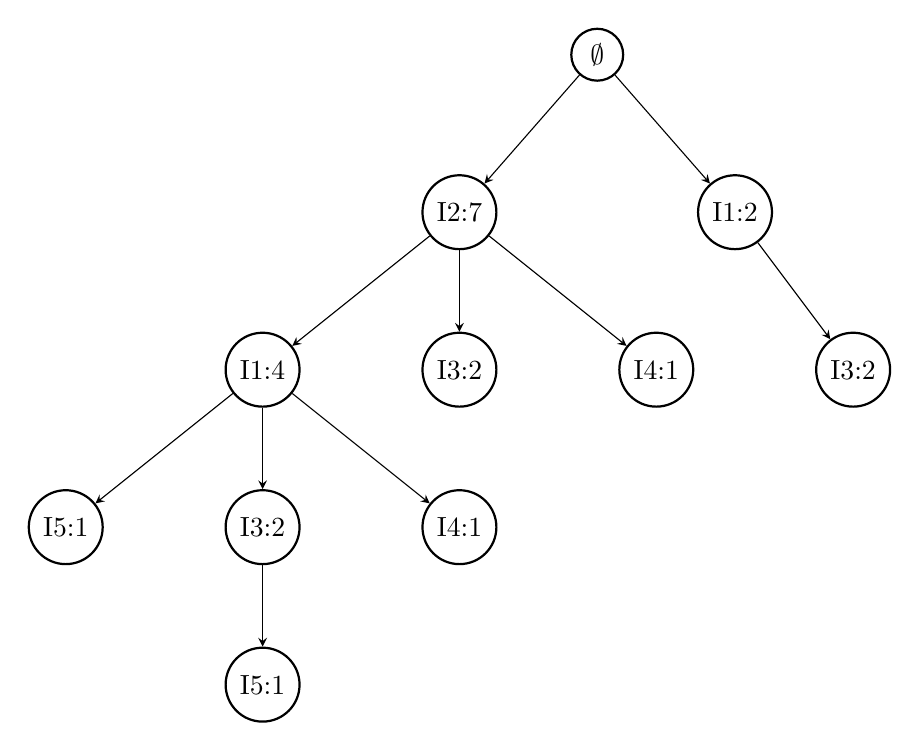
\begin{tikzpicture}[y=-1cm]
        \begin{scope}[every node/.style={circle,thick,draw}]
            \node (E) at (6.75,0) {$\emptyset$};
            \node (I2_7) at (5,2) {I2:7};
            \node (I1_2) at (8.5,2) {I1:2};
            \node (I3_2-first) at (5,4) {I3:2};
            \node (I1_4) at (2.5,4) {I1:4};
            \node (I4_1-first) at (7.5,4) {I4:1};
            \node (I3_2-second) at (10,4) {I3:2};
            \node (I5_1-first) at (0,6) {I5:1};
            \node (I3_2) at (2.5,6) {I3:2};
            \node (I4_1-second) at (5,6) {I4:1};
            \node (I5_1-second) at (2.5,8) {I5:1};
        \end{scope}
        \draw [-stealth] (E) -- (I2_7);
        \draw [-stealth] (E) -- (I1_2);
        \draw [-stealth] (I2_7) -- (I1_4);
        \draw [-stealth] (I2_7) -- (I3_2-first);
        \draw [-stealth] (I2_7) -- (I4_1-first);
        \draw [-stealth] (I1_2) -- (I3_2-second);
        \draw [-stealth] (I1_4) -- (I5_1-first);
        \draw [-stealth] (I1_4) -- (I3_2);
        \draw [-stealth] (I1_4) -- (I4_1-second);
        \draw [-stealth] (I3_2) -- (I5_1-second);
    \end{tikzpicture}
    \caption{The FP-Tree derived from scanning through the transactions.}
    \label{fig:fp-tree}
\end{figure}

Once the \acl{fpt} was created, we will move to the mining step of the algorithm.
This is the part where the divide and conquer part of the algorithm occurs.
We go through the collection $C$ in reversed order with each 1-itemset as a suffix pattern, create a \acl{cpb} of it, which is a sub-database of all the prefix patterns for the suffix pattern we are considering.
The reason we go through the collection $C$ in reversed order is because it will create good selectivity \citep{han2012mining}.
For examples, with the suffix pattern $I5$, it appears in two branches of the \acl{fpt} shown in \autoref{fig:fp-tree}: $\{I2, I1, I5: 1\}$ and $\{I2, I1, I3, I5: 1\}$.
Therefor, its \acl{cpb} will be $\{I2, I1: 1\}$ and $\{I2, I1, I3: 1\}$.
We then use the \acl{cpb} as a transactional database and formulate a \acl{cfpt} based on it.
The \acl{cfpt} is simply a single branch $\{I2:2, I1:2\}$ because $I3$ was filtered out since the support count of it is 1 which is smaller than the minimum support.
Now the task is to find all the combinations of \acl{cfpt} concatenating with the suffix then we will get the frequent patterns: $\{I2, I5: 2\}$, $\{I1, I5: 2\}$, $\{I2, I1, I5: 2\}$.
This will create a frequent pattern because both the suffix and the prefix are frequent.

We can see that we were able to find longer patterns from shorter ones, hence the name \textit{Frequent-Pattern Growth}.
By dividing the much larger database into smaller conditional databases, we were able to divide the problem recursively, which greatly reduced the complexity of the algorithm.
It has been found that the \acl{fpg} is an order of magnitude faster than the \acl{apriori} \citep{han2012mining}.

\section{Redescription mining}
\subsection{Definition}
Redescription mining is a process of discovering a set of criteria that describe a subset of data in multiple, complementary ways.
In other words, it is a method of coming up with various ways to describe the same data or set of data.
It can be used to find novel links or patterns in huge collections of data in a variety of domains.

\begin{figure}[bt]
    \centering
    \includegraphics[width=10cm]{niche-finding}
    \caption{An example redescription plotted on a map, showing the areas inhabited by lynxes (light red and medium purple) and the areas where the maximum March temperature is between \SI{-24.4}{\degreeCelsius{}} and \SI{3.4}{\degreeCelsius{}} (dark blue and medium purple) \cite{galbrun2018redescription}}
    \label{fig:niche}
\end{figure}
A classic example of redescription mining application is in finding bio-climatic niches, or, in other words, relate the habitat of particular species or groups of species, to the local climatic conditions.
In this example, we want to describe geographic regions in terms of the fauna that inhabits them, on one hand, and in terms of the values of some climatic variables, on the other hand. In particular, the aim of redescription mining is to extract such pairs of descriptions automatically from a given dataset.
As a specific example, the method might return a redescription that states that areas where the maximum temperature in March is between \SI{-24.4}{\degreeCelsius{}} and \SI{4.3}{\degreeCelsius{}} are roughly the same as area inhabited by lynxes (see Figure~\ref{fig:niche}).
In this application, the aim is to help ecologists understand the impact of climate on the distribution of species.

\begin{table}[tb]
    \resizebox{\textwidth}{!}{%
    \begin{tabular}{|l|l|l|l|l|l|l|l|l|l|l|l|}
    \cline{1-6} \cline{8-12}
    \multicolumn{6}{|c|}{Species occurrences} &  & \multicolumn{5}{c|}{Climate}                                  \\ \cline{1-6} \cline{8-12} 
    Location ID   & mountain hare & \dots & Canada lynx   & Eurasian lynx  & \dots  &  & Location ID & \dots & max.\ March T.\ & avg.\ May P.\ & \dots \\ \cline{1-6} \cline{8-12} 
    \dots  & \dots & \dots & \dots   & \dots  & \dots &  & \dots  & \dots & \dots & \dots & \dots \\ \cline{1-6} \cline{8-12} 
    4652 & True  & \dots & True  & False & \dots &  & 4652 & \dots & 2   & 10  & \dots \\ \cline{1-6} \cline{8-12} 
    4653 & True  & \dots & False & True & \dots &  & 4653 & \dots & 3   & 40  & \dots \\ \cline{1-6} \cline{8-12} 
    \dots. & \dots & \dots & \dots   & \dots  & \dots &  & \dots. & \dots & \dots & \dots & \dots \\ \cline{1-6} \cline{8-12} 
    \end{tabular}%
    }
    \caption{An example dataset, represented as a pair of data tables with mapped rows. The left-hand side table records occurrences of various species, while the right-hand side table records the values of various bio-climatic variables such as temperature (T, in \si{\degreeCelsius{}}) and precipitation (P, in \si{\milli\meter}).}
    \label{tab:mammals-and-climate}
\end{table}


Here we follow the formalism of \cite{Galbrun-Methods}.
The redescription mining data model $\mathcal{D}$ is a tuple of 3 sets: $\left( entity\;\mathcal{E}, attributes\;\mathcal{A}, views\;\mathcal{V} \right)$.
Each entity $e \in \mathcal{E}$ is associated with a set of attributes $a \in \mathcal{A}$.
The attributes are partitioned into disjoint \emph{views} $v \in \mathcal{V}$ that correspond to logical groups of attributes. Each view can be thought of as a data table, where the columns represent the attributes, and the rows represent the entities, which map across the different tables.
Usually, the data contains 2 datasets, one left-hand side and one right-hand side data.
In the bioclimatic-niche finding example above, the entities are geographic locations and the views correspond to species occurrences and climate, respectively.
That is, one view contains attributes that each record the presence or absence of a specific species in each location, whereas the other view contains attributes that each record the value taken by a specific climatic variable in each location.
This can be represented as a pair of tables, as shown in Table~\ref{tab:mammals-and-climate}.

Then, a description, or query, is a logical formula over attributes.
The query can be evaluated for each entity, and returns a Boolean value that indicates whether the entity satisfies the query conditions.
The support of a query is the set of entities that satisfy the query.
A redescription is then a pair of queries, respectively over attributes from distinct views, having sufficiently similar supports \cite{galbrun2018redescription}.
In the bioclimatic-niche finding example above, a redescription consists of a query over species occurrences and a query over climatic variables, respectively, that are satisfied in roughly the same locations.

For a redescription to satisfy the conditions, it must have similar supports between the two queries.
The similarity of the two queries $p$ and $q$ is denoted as $\sim$.
We can use the Jaccard distance to determine the similarity between the supports of the two description.
The Jaccard distance is based on the \acl{JSI}.

\begin{definition}[\acl{JSI} \citep{galbrun2018redescription}]
    The Jaccard (similarity) index J between the supports of two descriptions p and q is defined as below:

    \begin{equation}
        J(p, q) = J(supp(p), supp(q)) = \cfrac{\left|supp(p)\cap supp(q)\right|}{\left|supp(p)\cup supp(q)\right|}
    \end{equation}
\end{definition}

The requirement to calculate $J$ is obviously that none of $supp(q)$ and $supp(p)$ equals $\emptyset$.

\begin{definition}[Jaccard distance \citep{galbrun2018redescription}]
    The Jaccard distance is then defined as:

    \begin{equation}
        1 - J(p, q) = 1 - \cfrac{\left|supp(p)\cap supp(q)\right|}{\left|supp(p)\cup supp(q)\right|}
    \end{equation}
\end{definition}

Clearly, the smaller the distance is, the more accurate the redescription is.
When the distance between the two queries equals to $0$, the redescription is called \textit{exact}, and is denoted as $p \equiv q$.

From here, we can formulate the formal definition of the redescription.

\begin{definition}[Redescription \citep{galbrun2018redescription}]
    A redescription in query language $\mathcal{Q}$ over data $\mathcal{D}$ with similarity $\sim$ is a pair of query $(p, q) \in \mathcal{Q} \times \mathcal{Q}$ such that

    \begin{equation}
        p \sim q \text{ and } views(p) \cap views(q) = \emptyset
    \end{equation}
\end{definition}

\subsection{Redescription mining algorithms}
Different redescription mining algorithms have been proposed, that use different strategies, handle different types of attributes and allow different types of constraints on the queries \cite{galbrun2018redescription}.
There are two main categories of redescription mining algorithms: exhaustive and heuristic.
In the scope of the current thesis, we will be focusing on the exhaustive algorithms.

The most popular strategy of exhaustive redescription mining algorithms is \ac{MAP}.
The idea is quite simple, first we mine for all possible queries, then we will try to pair them together and see if their supports have big enough overlaps.
If the overlap between the two queries is bigger than a certain threshold, we then have found a redescription.

The \ac{MID} algorithm is an algorithm that follow the \ac{MAP} strategy.
We can have a look at the pseudocode of the \acl{MID} in Algorithm \ref{alg:MID}.
The mining for queries steps is in line 2, where the paring part is at line 12.

Recall that in statistic, p-value is the probabilities of the null hypothesis to be true.
The null hypothesis in this case is that the supports of a query is small.
The reason this is the hypothesis is that the chance of two disjoint small support sets to have overlap are small.

\begin{algorithm}[tb]
    \caption{Sketch of the \algMID{} algorithm \citep{galbrun2018redescription}.}
      \label{alg:MID}
    \begin{algorithmic}[1]
    \small
      \Require Two Boolean data tables $\Table_1$ and $\Table_2$, similarity $\similar$, maximum \pvalue{} $p_{\max}$, number of queries to select $N$, and maximum level $\kappa$.
      \Ensure Redescriptions $\mathcal{R}$.
      \For{side $i \in \{1, 2\}$} %\Comment{for each view separately}
       \State $\Queries^{(0)}_i \gets \{ \query : \query$ is a closed frequent itemset from $\Table_i$ or its negation and $ \pvalue(\query) \leq p_{\max}\}$ \label{alg:MID:mine} %\Comment{computing the \pvalue{} for the independent items \textit{null-model}}
       \State $\Queries^{(1)}_i \gets$  $N$ queries with the lowest \pvalue from $\Queries^{(0)}_i$ 
       \For{level $k \in \{1,\dots,(\kappa-1)\}$}
         \State $\Queries^{(k+1)}_i \gets \Queries^{(k)}_i$
         \For{operator $\lop \in \{\land, \lor\}$} % \Comment{combine queries using conjunctions and disjunctions}
            \State $\Queries^{(k+1)}_i \gets \Queries^{(k+1)}_i \cup \{ \query \lop \query' : \query, \query' \in \Queries^{(k)}_i, \pvalue(\query \lop \query') \leq p_{\max}\}$ \label{alg:MID:combine}
      \EndFor
       \State $\Queries^{(k+1)}_i \gets$  $N$ queries with the lowest \pvalue from $\Queries^{(k+1)}_i$ \label{alg:MID:filter}
      \EndFor
      \EndFor
      \State $\mathcal{R} \gets \{(\lquery, \rquery) \in \Queries^{(\kappa)}_1 \times \Queries^{(\kappa)}_2  : \lquery \similar \rquery\}$ \label{alg:MID:pair} %\Comment{collect query pairs across the views with sufficient accuracy}
      \State \textbf{return} $\mathcal{R}$
    \end{algorithmic}
\end{algorithm}

We can see that the \acl{arm} algorithms contribute an important part of the foundation of this redescription mining algorithm category.
Often times, a suitable \ac{fim} algorithms is the key to create a redescription mining algorithm for a specific problem.
For example the CHARM-L \citep{zakihsiao2005}, which is a \ac{fim} algorithm that can construct the closed itemset lattice.
The CHARM-L algorithm was then utilized to develop a redescription mining algorithm to find the exact conditional redescriptions for the lattice \Citep{zakimohammed2005}.
In the paper, three classes of redescription was formulated: exact, conditional, and approximate.
An exact redescription has a Jaccard distance = 0, while an approximate redescription has a Jaccard distance > 0.
A conditional redescription is derived from an approximate redescription and turned into an exact redescription by supplying additional constraints to the queries.
For instance, we have 2 queries $p$ and $q$ forming a redescription $(p \similar q)$ with a Jaccard distance distance > 0.
By introducing an additional constraint to both queries: $(p \cap r)$ and $(p \cap r)$, $(p \cap r) \similar (p \cap r)$ could have a Jaccard distance = 0.
This is denoted by $(p \similar q \mid r)$ where $p$, $q$, and $r$ are queries over some disjoint view $v \in \mathcal{V}$.


\chapter{Employing ECLAT for Redescription Mining}
\label{cha:employment}
\section{Mine and Pair}
\section{Mine and Split}

\chapter{Experiments}
\label{cha:experiments}

\chapter{Conclusions}
\label{cha:conclusions}